\documentclass{article}

\usepackage{amsmath, amsthm, amssymb, amsfonts}
\usepackage{thmtools}
\usepackage{graphicx}
\usepackage{setspace}
\usepackage{geometry}
\usepackage{float}
\usepackage{hyperref}
\usepackage{enumitem}

\usepackage[utf8]{inputenc}
\usepackage[english]{babel}
\usepackage{framed}
\usepackage[dvipsnames]{xcolor}
\usepackage{tcolorbox}

\colorlet{LightGray}{White!90!Periwinkle}
\colorlet{LightOrange}{Orange!15}
\colorlet{LightGreen}{Green!15}

\newcommand{\HRule}[1]{\rule{\linewidth}{#1}}

\declaretheoremstyle[name=Theorem,]{thmsty}
\declaretheorem[style=thmsty,numberwithin=section]{theorem}
\tcolorboxenvironment{theorem}{colback=LightGray}

\declaretheoremstyle[name=Proposition,]{prosty}
\declaretheorem[style=prosty,numberlike=theorem]{proposition}
\tcolorboxenvironment{proposition}{colback=LightOrange}

\declaretheoremstyle[name=Principle,]{prcpsty}
\declaretheorem[style=prcpsty,numberlike=theorem]{principle}
\tcolorboxenvironment{principle}{colback=LightGreen}

\setstretch{1.2}
\geometry{
    textheight=9in,
    textwidth=5.5in,
    top=1in,
    headheight=12pt,
    headsep=25pt,
    footskip=30pt
}

% ------------------------------------------------------------------------------

\begin{document}

% ------------------------------------------------------------------------------
% Cover Page and ToC
% ------------------------------------------------------------------------------

\title{ \normalsize \textsc{}
		\\ [2.0cm]
		\HRule{1.5pt} \\
		\LARGE \textbf{\uppercase{UML II - interdisciplinary assignment}
		\HRule{2.0pt} \\ [0.6cm] \LARGE{Case: Big Mamma pizzaria} \vspace*{10\baselineskip}}
		}
\date{}
\author{\textbf{Jonas Smidt} \\ 
		Hold: rf24daf1-1fDAT-1F \\
		\textit{Zealand Roskilde}
  }

\maketitle
\newpage

\tableofcontents
\newpage

% ------------------------------------------------------------------------------
\section{User Stories and Acceptance Criteria}

 The following user-stories and acceptance criteria was based upon the scenario-based template From the following website\cite{knuthwebsite}




\subsection{Customer Administration}

\begin{enumerate}[label= \textbf{User Story \arabic*:}]
    \item \textbf{As a} manager,\\
    \textbf{I want to} make a list of customers,\\
    \textbf{So that} I can keep track of all customers registered in the system.
    
    \textbf{Acceptance Criteria:}
    \begin{itemize}
        \item \textbf{Given} a list of registered customers,\\
        \textbf{That} the system provides an option to view all customers,\\
        \textbf{Then} the system displays a comprehensive list including customer names, contact information, and addresses.
    \end{itemize}
\end{enumerate}

% Add other user stories and acceptance criteria similarly

\subsection{Pizza Menu Administration}

\begin{enumerate}[resume, label= \textbf{User Story \arabic*:}]
    \item \textbf{As a} manager,\\
    \textbf{I want to} create, delete, and update a pizza,\\
    \textbf{So that} I can maintain an updated menu for the customers.
    
    \textbf{Acceptance Criteria:}
    \begin{itemize}
        \item \textbf{Given} pizza details provided by the manager,\\
        \textbf{That} the system offers options to create, delete and update a pizza,\\
        \textbf{Then} the system executes the respective action as requested and provides confirmation of the action taken.
    \end{itemize}
\end{enumerate}

% Add other user stories and acceptance criteria similarly

\subsection{Order Administration}

\begin{enumerate}[resume, label= \textbf{User Story \arabic*:}]
    \item \textbf{As a} manager,\\
    \textbf{I want to} create, delete, and update an order,\\
    \textbf{So that} I can efficiently manage customer orders.
    
    \textbf{Acceptance Criteria:}
    \begin{itemize}
        \item \textbf{Given} order details provided by the manager,\\
        \textbf{That} the system offers options to create, delete, and update an order,\\
        \textbf{Then} the system executes the respective action as requested and provides confirmation of the action taken.
    \end{itemize}
\end{enumerate}

% Add other user stories and acceptance criteria similarly
\newpage
\subsection{Menu displaying}

\begin{enumerate}[resume, label= \textbf{User Story \arabic*:}]
    \item \textbf{As a} user,\\
    \textbf{I want the system to} print out a menu on the screen,\\
    \textbf{So that} I can easily navigate the available options.
    
    \textbf{Acceptance Criteria:}
    \begin{itemize}
        \item \textbf{Given} a request to view the menu,\\
        \textbf{That} the system provides a menu display functionality,\\
        \textbf{Then} the system prints a menu on the screen with clearly labeled options.
    \end{itemize}
\end{enumerate}

\subsection{Customer Administration}

\begin{enumerate}[resume, label= \textbf{User Story \arabic*:}]
    \item \textbf{As a} manager,\\
    \textbf{I want to} search for a customer based on name,\\
    \textbf{So that} I can quickly access and manage specific customer information.
    
    \textbf{Acceptance Criteria:}
    \begin{itemize}
        \item \textbf{Given} a search query for a customer's name,\\
        \textbf{That} the system provides a search functionality,\\
        \textbf{Then} the system displays relevant customer information matching the search criteria.
    \end{itemize}
\end{enumerate}

% Add other user stories and acceptance criteria similarly

\subsection{Pizza Menu Administration}

\begin{enumerate}[resume, label= \textbf{User Story \arabic*:}]
    \item \textbf{As a} manager,\\
    \textbf{I want to} print out on the screen a list of pizzas,\\
    \textbf{So that} I can easily review the available options.
    
    \textbf{Acceptance Criteria:}
    \begin{itemize}
        \item \textbf{Given} a request to view the pizza menu,\\
        \textbf{That} the system provides an option to print a list of all pizzas,\\
        \textbf{Then} the system displays a list that includes pizza names, toppings, and prices.
    \end{itemize}
\end{enumerate}

% Add other user stories and acceptance criteria similarly

\subsection{Order Administration}

\begin{enumerate}[resume, label= \textbf{User Story \arabic*:}]
    \item \textbf{As a} manager,\\
    \textbf{I want to} make a list of orders,\\
    \textbf{So that} I can keep track of all orders received.
    
    \textbf{Acceptance Criteria:}
    \begin{itemize}
        \item \textbf{Given} a list of orders,\\
        \textbf{That} the system provides an option to view all orders,\\
        \textbf{Then} the system displays a comprehensive list including order details such as order ID and customer name.
    \end{itemize}
\end{enumerate}

% Add other user stories and acceptance criteria similarly
\newpage
\subsection{Multi selection of pizza toppings}
\begin{enumerate}[resume, label= \textbf{User Story \arabic*:}]
    \item \textbf{As a} User,\\
    \textbf{I want to} choice between different pizza toppings,\\
    \textbf{So that} I can eat different types of pizzas.
    
    \textbf{Acceptance Criteria:}
    \begin{itemize}
        \item \textbf{Given} a list of pizza toppings ,\\
        \textbf{That} the system provides an option to view all pizza types,\\
        \textbf{Then} the system displays a list of different kinds of pizzas.
    \end{itemize}
\end{enumerate}

\subsection{Payment confirmation}
\begin{enumerate}[resume, label= \textbf{User Story \arabic*:}]
    \item \textbf{As a} Customer,\\
    \textbf{I want to} pay for my pizza,\\
    \textbf{So that} I can feel at ease.
    
    \textbf{Acceptance Criteria:}
    \begin{itemize}
        \item \textbf{Given} that i am registered as an customer,\\
        \textbf{That} the system provides an option to insert the amount of money,\\
        \textbf{Then} the system displays the amount paid for the pizza.
    \end{itemize}
\end{enumerate}


\subsection{Error handling}

\begin{enumerate}[resume, label= \textbf{User Story \arabic*:}]
    \item \textbf{As a} user,\\
    \textbf{I want the system to} handle errors in the input,\\
    \textbf{So that} I can navigate through the system smoothly without encountering issues.
    
    \textbf{Acceptance Criteria:}
    \begin{itemize}
        \item \textbf{Given} invalid user input,\\
        \textbf{That} the system detects errors,\\
        \textbf{Then} the system provides clear error messages guiding the user on how to correct their input or select alternative options.
    \end{itemize}
\end{enumerate}
\newpage
\section{Domain model}
\subsection{Why Domain models}
Domain models are purely conceptualized and used in the process before coding to act as a \textit{"source of inspiration for designing some software objects".}(Larman, 2004)
\cite{larman2004applying}


\subsection{Big Mamma Pizza Domain model}
\begin{figure}[htbp]
    \center
    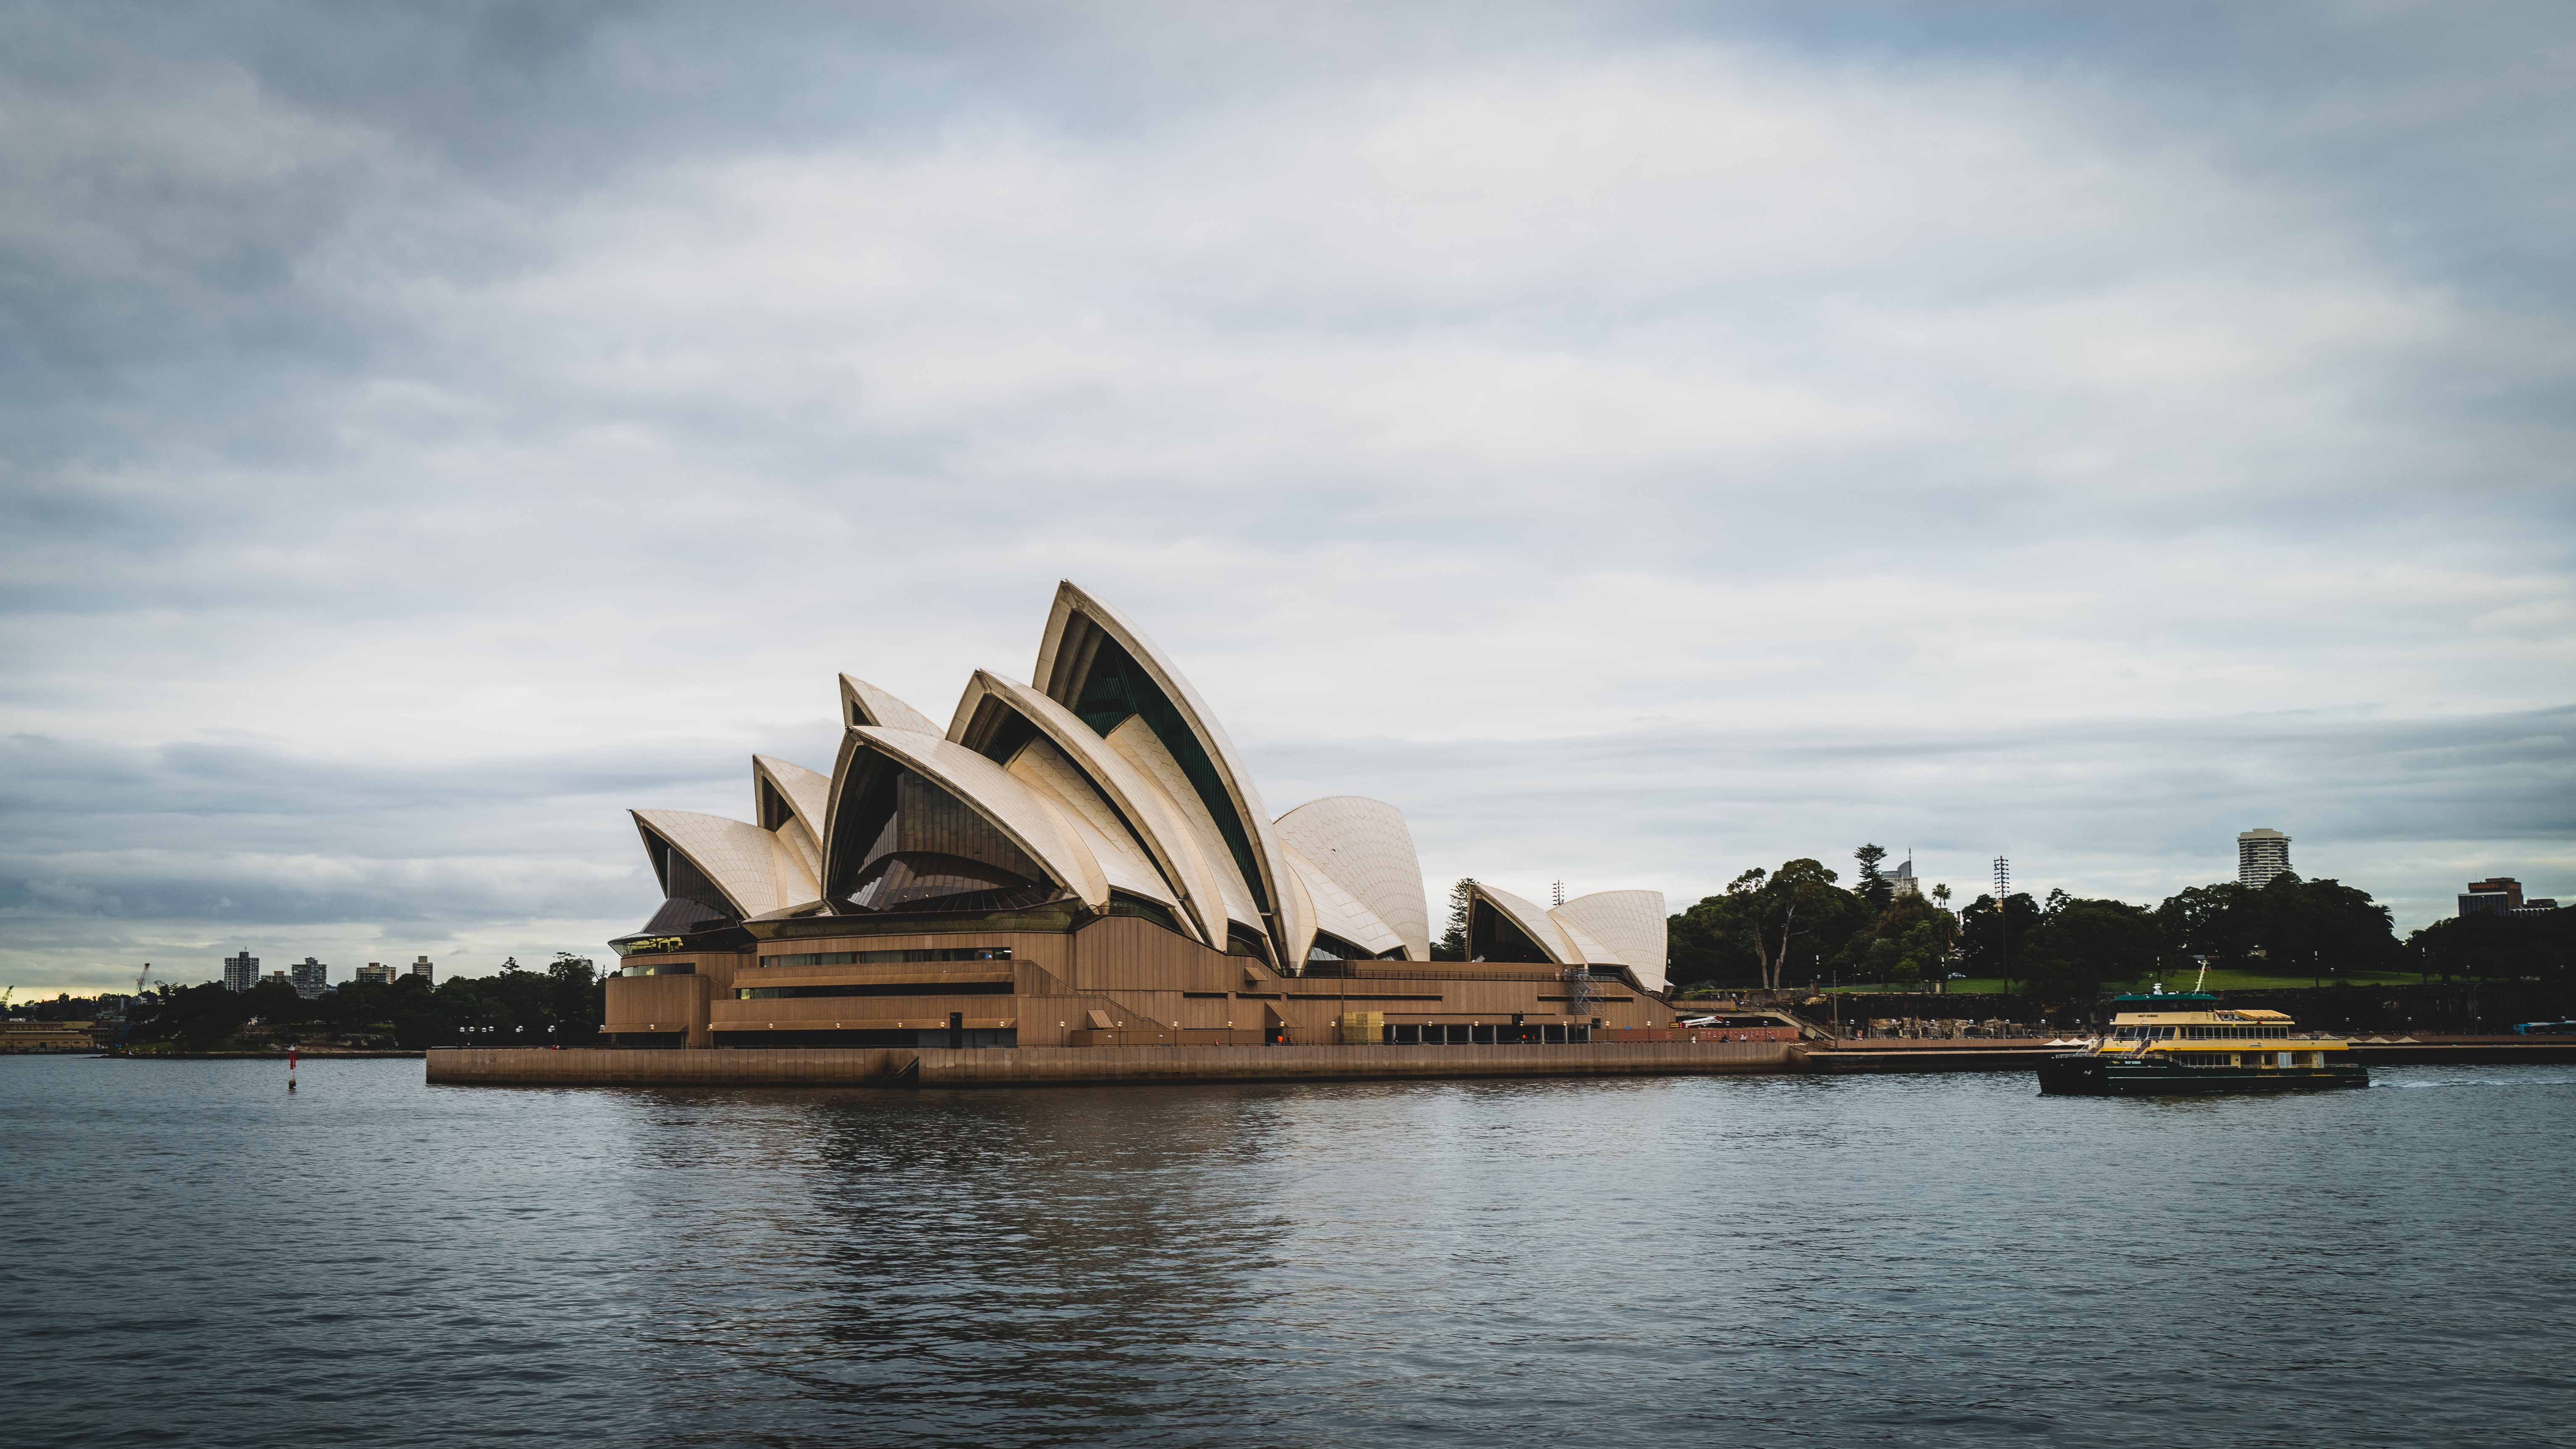
\includegraphics[scale=0.07]{img/photo.jpg}
    \caption{}
\end{figure}



\newpage
\section{Design Class Diagram}



\begin{figure}[htbp]
    \center
    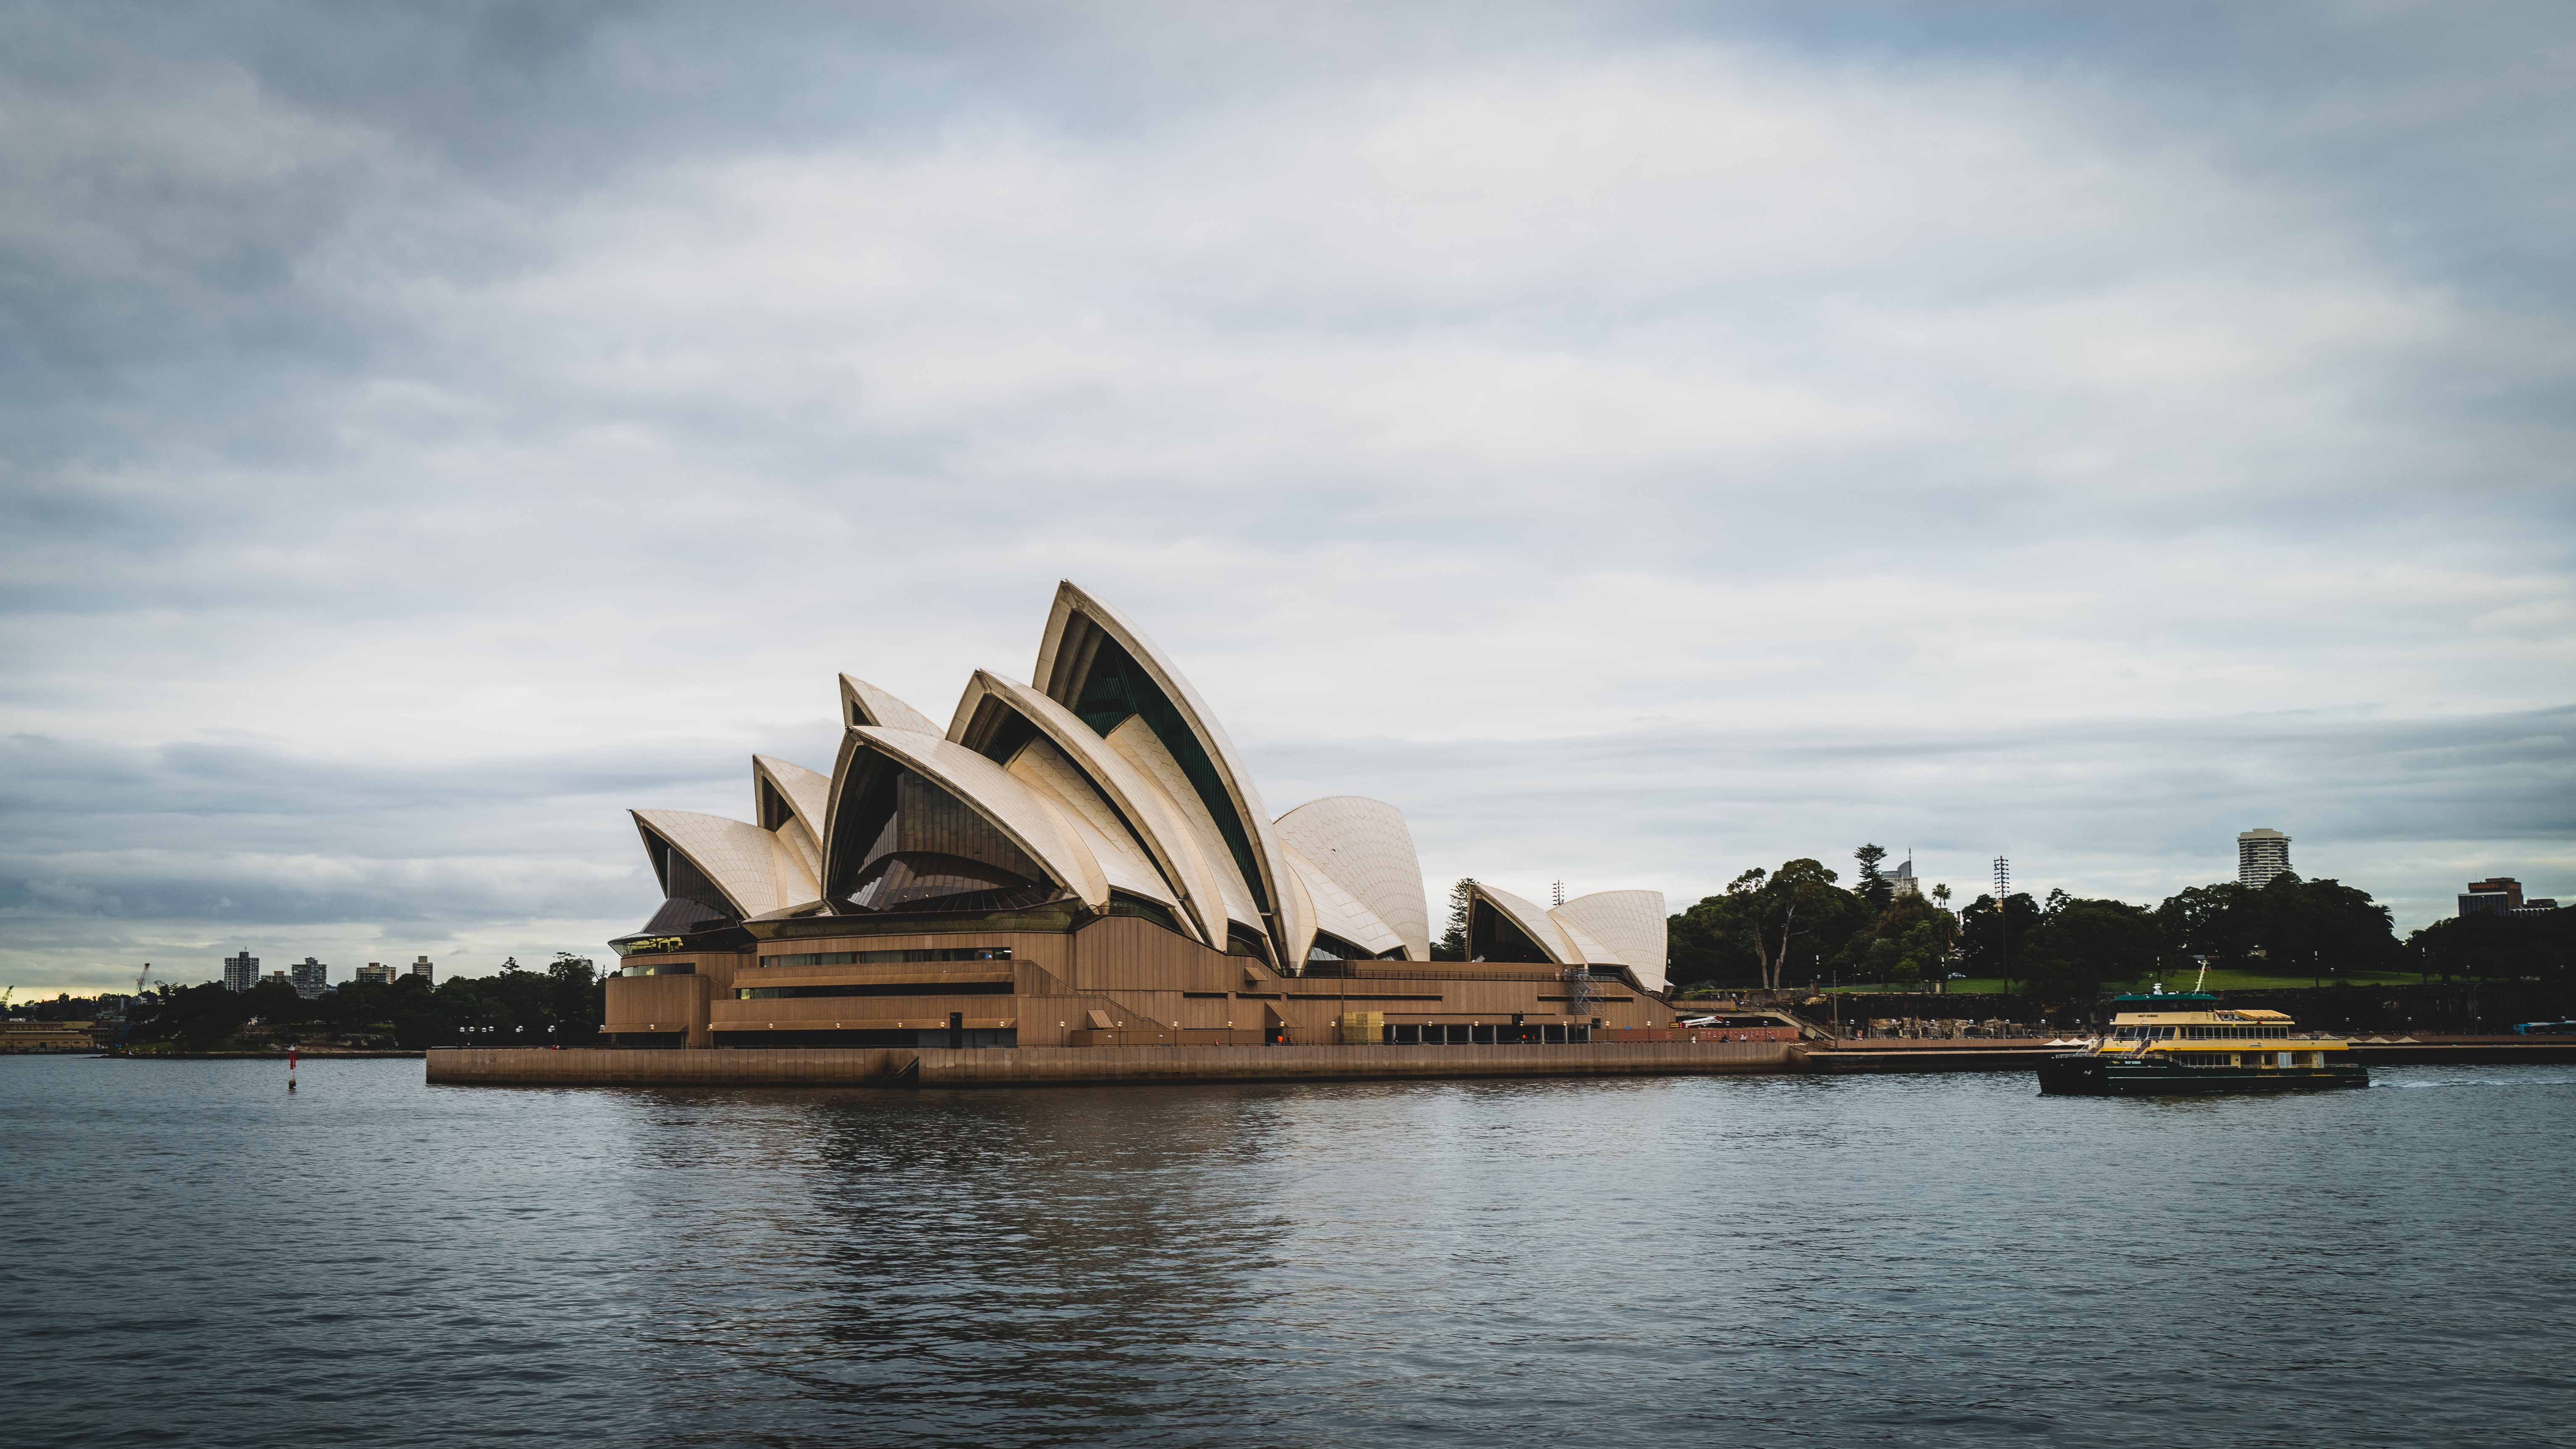
\includegraphics[scale=0.07]{img/photo.jpg}
    \caption{}
\end{figure}



\newpage
\section{Sequence Diagram}

\begin{figure}[htbp]
    \center
    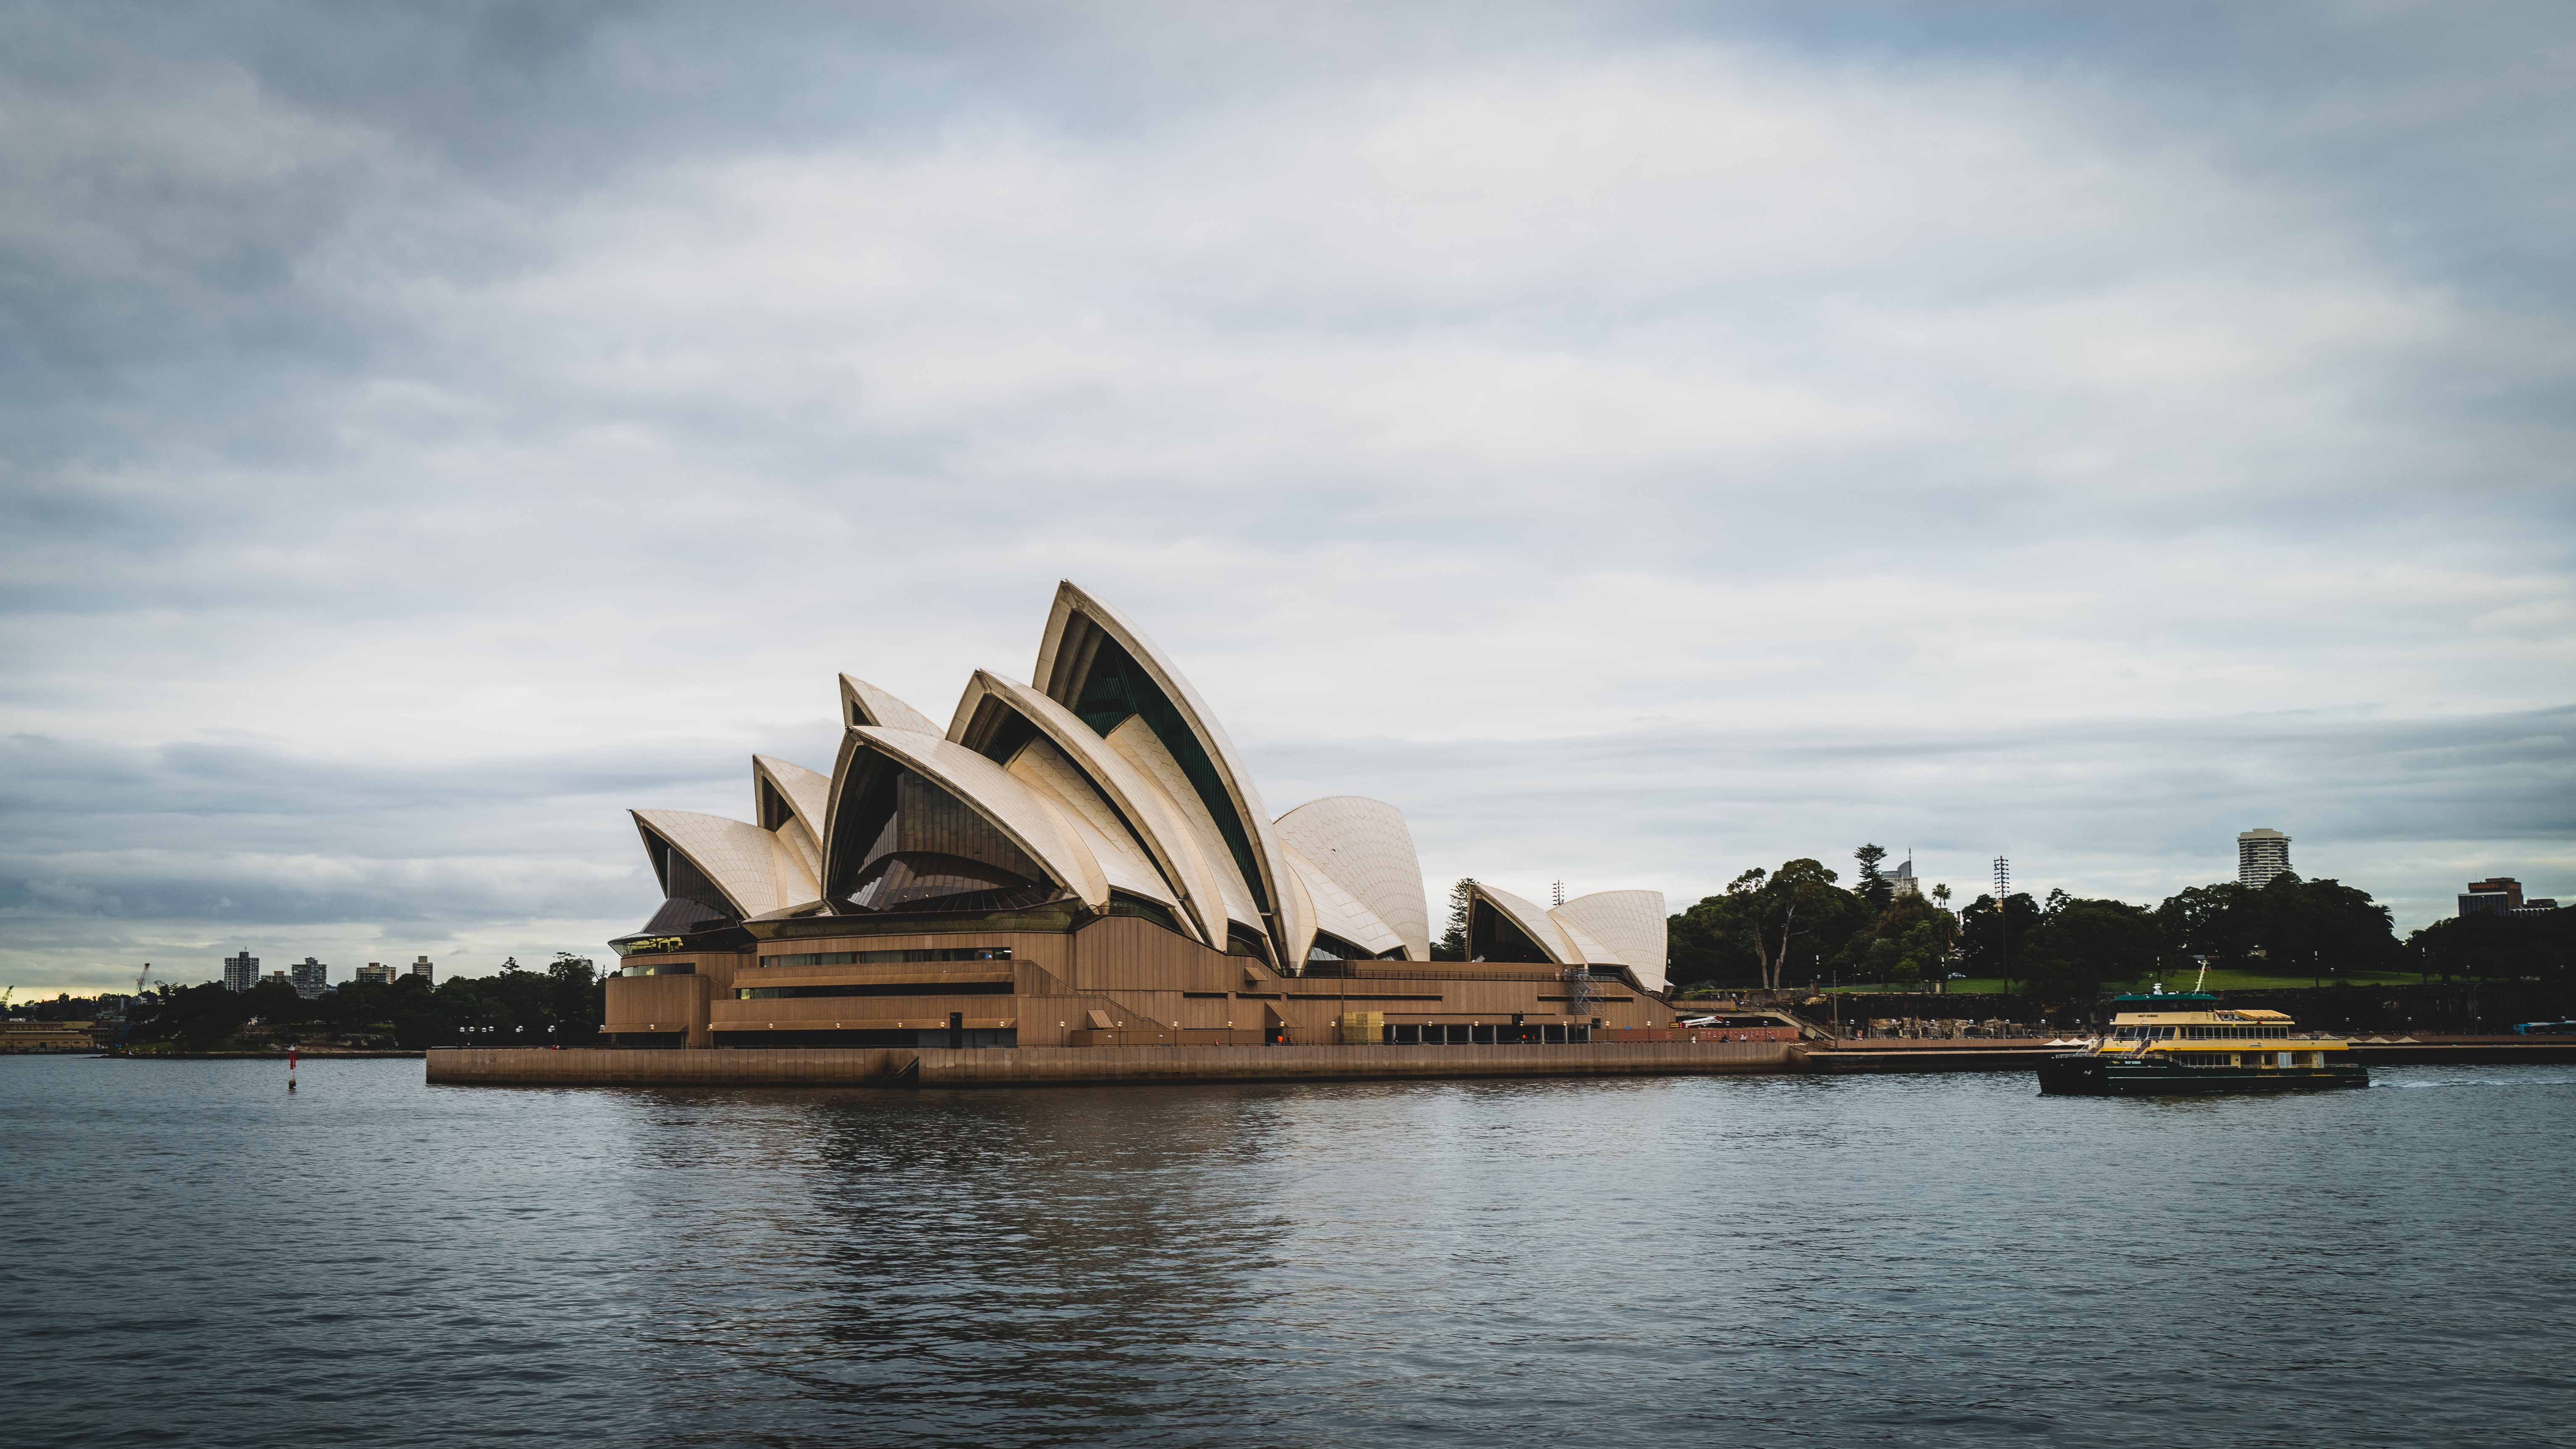
\includegraphics[scale=0.07]{img/photo.jpg}
    \caption{Text}
\end{figure}


\newpage
\section{Implement Design Class}


Click \href{https://github.com/Josmanid/PizzaStore}{\textbf{Here!}} to access my GitHub project.

\newpage



% ------------------------------------------------------------------------------
% Reference and Cited Works
% ------------------------------------------------------------------------------

\bibliographystyle{IEEEtran}
\bibliography{References.bib}

% ------------------------------------------------------------------------------

\end{document}
